\section{Introduction}
People with a visual impairment are not able to read text or reliably interpret visual input. For this target group special types of books, such as braille or audio books, are made to enable these people to still perform the same task but then via a different medium. 

Similarly, user interfaces of programs on computers are often enhanced in such a way that screen readers (text-to-speech software) can easily read out what is being displayed on the screen. Examples of these enhancements are alternative texts for images or reorganizing the layout such that only relevant information is given to the screen reader. However, in a study about the frustrations of screen reader users on the web \citeauthor{lazar2007frustrates} \cite{lazar2007frustrates} aggregated a list of causes of frustration from 100 blind users. This list showed that the often used enhancements, such as alternative text for images, are not always used on websites. The top causes of frustrations include (among others) the layout that causes out of order auditory output from the screen reader, poorly designed forms and no alternative text for images. 

The study about the frustrations of screen reader users on the web shows that one cannot rely on websites to provide a user friendly experience, such as a well formatted layout or an additional description of the images. In collaboration with the foundation Dedicon, which is involved in producing braille and audio books, this thesis will mainly focus on enhancing images with relevant textual descriptions. A few examples of what Dedicon already takes care of are the layout of magazines, which will influence the reading order of the screen readers, or school books that are manually edited to make them more accessible for visual impaired people by changing assignments that refer to images. Currently, important images are manually enhanced or replaced with text and this thesis takes a step into automating this process by augmenting current state-of-the-art image annotation techniques with textual context. Multiple fields within artificial intelligence, such as computer vision, machine learning and linguistics, can be used to help the end-user with providing a computer generated description of an image. 

The research question that will be answered in this thesis is twofold. The primary question is: `Does textual context in which an image is present contribute to the performance of automatically generating a description?'. However, the main emphasis lies on the secondary question: `If so, how can textual context be integrated into a multimodal Recurrent Neural Network model?'

In Section~\ref{sec:methods} the methods of the study is described in more detail. The results of this study are depicted in Section~\ref{sec:results} and the last two sections, Section~\ref{sec:discussion} and \ref{sec:conclusion}, discuss these results and draw a general conclusion from them.

The next section provides more clarity of the concept textual context that is used throughout this thesis. The following sections give more background information on the current state-of-the-art in the computer vision field concerning object detection and classification as well as the latest models regarding image description generation.


\subsection{Textual context}
\label{sec:textual-context}
Before going into more detail of previous studies, first some clarification on the definition of textual context that will be used in the rest of this thesis.

In linguistics context refers to the commonality of implicit information between sentences. In \cite{Fortu2005} this is exemplified with the following pair of sentences:

\begin{displayquote}
	\emph{``John got a new job on Monday. He got up early, shaved, put on his best suit and went to the interview.''}
\end{displayquote}

\noindent Here the common information is the temporal information about the day that is explicitly available in the first sentence,  whereas the second sentence does not state this information. However, the temporal information is still implicitly available in the second sentence due to context. 

A similar process seems to be involved around textual context in combination with images. Often an image is surrounded by text that is related to one or more objects or even relations between objects in the image. This textual context could give an additional semantic meaning which cannot be distilled from having solely the image. Examples of such additional meaning are names of objects (e.g. people, animals), place or resolving ambiguity (e.g. partial objects) in an image. Textual context versus no textual context of an arbitrary image is depicted in Figure~\ref{fig:textual-context}. Without the surrounding text (Figure~\ref{fig:wo-textual-context}), the only sensible text that can describe the image could involve the words \emph{$\{$red cat, sitting, stone, grass, looking$\}$}. 

However, when a context (Figure~\ref{fig:w-textual-context}) is introduced this changes the meaning of the image, since the red cat now has a name as well as the object which the cat sits on top of and more sensible words can be used \emph{$\{$Tigger, sitting, bench, grass, looking$\}$}. Even though this is a toy example, this illustrates the importance of context especially for visually impaired people where a general description might not be informative enough.

Thus, more formally textual context w.r.t. this thesis is:

% TODO: Improve this definition
\begin{displayquote}
	\emph{Words or sentences that provide explicit information that can be used to support or alter the implicit information of an image}.
\end{displayquote}

\begin{figure}[h!]
\centering
	\begin{subfigure}[b]{0.3\textwidth}
		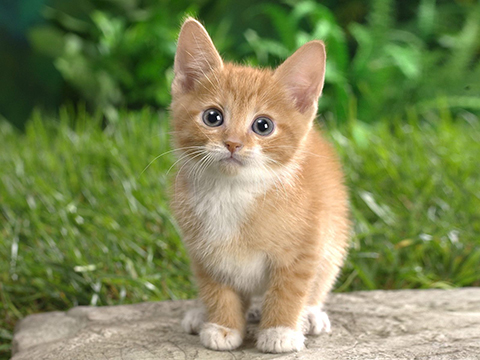
\includegraphics[width=\textwidth]{images/cat}
		\caption{}
		\label{fig:wo-textual-context}	
	\end{subfigure}\quad\quad
	\begin{subfigure}[b]{0.4\textwidth}
		% Generate irregular line: 
		% http://tex.stackexchange.com/questions/143070/drawing-randomly-ragged-lines-in-technical-drawings
		\newcommand\irregularline[2]{%
		  let \n1 = {rand*(#1)} in
		  +(0,\n1)
		  \foreach \a in {0.1,0.2,...,#2}{
		    let \n1 = {rand*(#1)} in
		    -- +(\a,\n1)
		  }  
		} % #1=seed, #2=length of horizontal line
		
		\begin{tikzpicture}
			\node at 		(1,0.6) {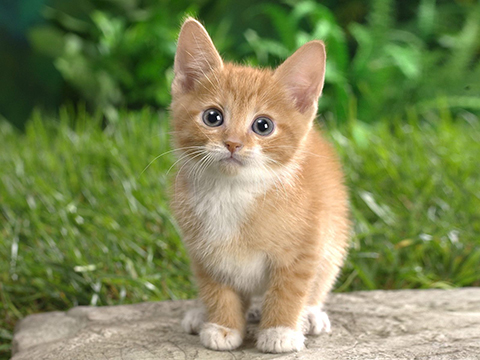
\includegraphics[width=0.4\textwidth]{images/cat}};
			\draw[black] 	(0,2) \irregularline{1mm}{1.5};
			\node[draw] at 	(2.5,2) {Tigger};
			\draw[black] 	(3.5,2) \irregularline{1mm}{2};
			\draw[black]		(2.5,1.5) \irregularline{1mm}{3};
			\draw[black]		(2.5,1)	\irregularline{1mm}{1.5};
			\node[draw] at	(4.8,1) {sitting};
			\draw[black]		(2.5,0.5) \irregularline{1mm}{3};
			\draw[black]		(2.5,0) \irregularline{1mm}{3};
			\node[draw] at	(0.6,-0.8) {bench};
			\draw[black]		(1.5,-0.8) \irregularline{1mm}{1.5};
			\node[draw] at	(4,-0.8) {looking};
			\draw[black]		(5,-0.8) \irregularline{1mm}{0.5};
			
		\end{tikzpicture}
		\caption{}
		\label{fig:w-textual-context}
	\end{subfigure}
\caption{Figure~\ref{fig:wo-textual-context} shows an arbitrary image without further textual context, whereas an illustration of that same image place within textual context is depicted in Figure~\ref{fig:w-textual-context}. Candidate keywords are highlighted in the rest of the scribbled context.}
\label{fig:textual-context}
\end{figure}

% TODO: include studies??


\subsection{Background}
Multiple studies use context to categorize \cite{Rabinovich2007, carbonetto2004statistical}, segment \cite{Sande2011} or describe \cite{mao2015learning} objects or images each with their own application of context. For categorization the context in which the detected objects are present is useful to eliminate out of place labeled objects. Entirely different, for describing and segmenting objects or images context of lower-level features is used to improve the task at hand.

In light of textual context, \citeauthor{mao2015learning} \cite{mao2015learning} harness the idea of novel concepts to improve generated image descriptions for the Novel Visual Concept learning from Sentences (NVCS) task. The core idea here is to extend a pre-trained base model with the capability to update certain concepts, that are already trained on a large dataset, with novel concepts. These novel concepts, which are image-sentence pairs, are included in a small dataset. With limited amount of learning, their model can improve the base model. Throughout the paper an example is used involving the novel Harry Potter concept \emph{quidditch}; the base model would describe an image depicting such a concept with the following sentence:

\begin{displayquote}
	\emph{``A group of people playing a game of soccer''}
\end{displayquote}

After a learning session of 100 image-sentence pairs involving quidditch, the same example image now results in:

\begin{displayquote}
	\emph{``A group of people is playing quidditch with a red ball''}
\end{displayquote}

The approach of NVCS can be seen as augmenting the generalized model with novel concepts and falls in the definition given in Section~\ref{sec:textual-context}. Here, presenting novel concepts can be seen as  providing explicit information of what is depicted on an image. The upside of their approach is that original concepts are not disturbed. However, this process is not one-shot learning, since multiple image-sentence pairs are used. Furthermore, in order to improve other concepts that are incorrectly described, a dataset per concept is required.

Literature shows many studies involving object recognition and classification \cite{carbonetto2004statistical, he2015delving} using Convolutional Neural Networks (CNNs). In these studies objects ranging from inanimate to animate in images are classified, which results in a label that describes to which class each object belongs to. One of the more recent studies \cite{he2015delving} claims a performance that even surpasses human performance on classifying images from the ImageNET dataset \cite{russakovsky2014imagenet}. While this study focuses on the image classification by labeling images, other studies \cite{mao2014explain, mitchell2012midge, Yang2011, Farhadi2010} have focused on the generation of sentences from images by combining a computer vision approach with linguistic models. 

For description generation often two types of approaches are used in the literature. The first type is connecting the grammar of a sentence in a description to an object or a relation between objects \cite{karpathyjoulin2014deep, Farhadi2010}. Models that use this approach generate sentences for the description that are following the syntactically correctness of the language grammar. The description generation model that is mentioned in \cite{mitchell2012midge} follows this first approach. It is trained on the Flickr datasets which consists of images and descriptions. In order to generate meaningful sentences, the model uses co-occurrence statistics to compute the probability distribution within a noun phrase. Furthermore, the characteristics of visually descriptive text are inspected to determine what generally the structure is of this type of text. These statistics are then used in the model along with the computer vision input (number of objects, labels) to generate novel sentences.

The second type of approach is using probabilistic machine learning to learn the probability density over multimodal input such as text and images. These models also generate sentences for the description, but are not necessarily according to a grammar. This results into more expressive sentences, but may contain less sound grammatical structures. The models in \cite{mao2014explain,karpathyfeifei2014deep,karpathyjoulin2014deep} are according to this second approach and the authors describe the model which consists of a multimodal Recurrent Neural Network. What this network makes multimodal network is the multimodal layer. This layer connects the word representations layer with the image feature extraction network that is finally combined into a multimodal feature vector. 

In this taxonomy of approaches for description generation, this thesis fits into the latter approach where multimodal input is used to learn a probability density over image-description pairs.

\subsection{Base model}
The base model that will be used is based on the model by \citeauthor{karpathyfeifei2014deep} where a CNN is combined with either a Recurrent Neural Network \cite{karpathyfeifei2014deep} or a Long-Short Term Memory (LSTM) network \cite{vinyals2014show}. Both approaches use a CNN by \citeauthor{simonyan2014very} \cite{simonyan2014very} to extract features from an image and a model which can integrate the image features and a sequence of words.  

When an LSTM model is compared to an RNN model an LSTM model tends to outperform the other model on sequence tasks such as generating sentences from images or translation \cite{vinyals2014show}. 
% TODO: Extend this part

In the next sections the CNN is explained in more detail as well as the LSTM approach for combining the image and text.

\subsubsection{Image features}
The CNN part of the multimodal model is designed by \citeauthor{simonyan2014very}. They participated in the ImageNet Large-Scale Visual Recognition Challenge (ILSVRC) 2014 as the Visual Geometry Group (VGG) with a very deep convolution network and finished with the first and second place. Prior to their work, CNNs mainly were shallow and consisted of only a few layers and convolution filters with large receptive fields were used. However, \citeauthor{simonyan2014very} took a different approach by lowering the size of the convolution filters to 3\texttimes 3 in all layers and by increasing the number of weight layers to 16 or 19. These architectures were not only able to achieve state-of-the-art accuracy on the classification and localization tasks, but were also able to generalize to other datasets.

The last layer of the model has 1000 output units that represent the 1000 categories on which the model has been trained. The activation of those units is the probability density for the categories to be present in the image. 

In order to integrate this model in the overall multimodal model, the classification layers are stripped off to expose the rectified linear unit (ReLU) in order to get the more rich internal representation of 4096 abstract features. Together with the text this is the input for the LSTM model.

\subsubsection{Combining image and text}
\citeauthor{vinyals2014show} use an LSTM model to generate sentences from images. The main component of such a model is the memory cell which contains information at every time step about the inputs that have been given up until this point of time. Furthermore, three binary gates govern the behavior of the model by telling the cell to forget the current value, read its input and outputting its new value. A general overview of such a model is shown in Figure~\ref{fig:lstm} where each part itself and the relation with other parts are depicted. The $\odot$ nodes indicate a multiplication with the gate values.

\begin{figure}[h!]
\centering
	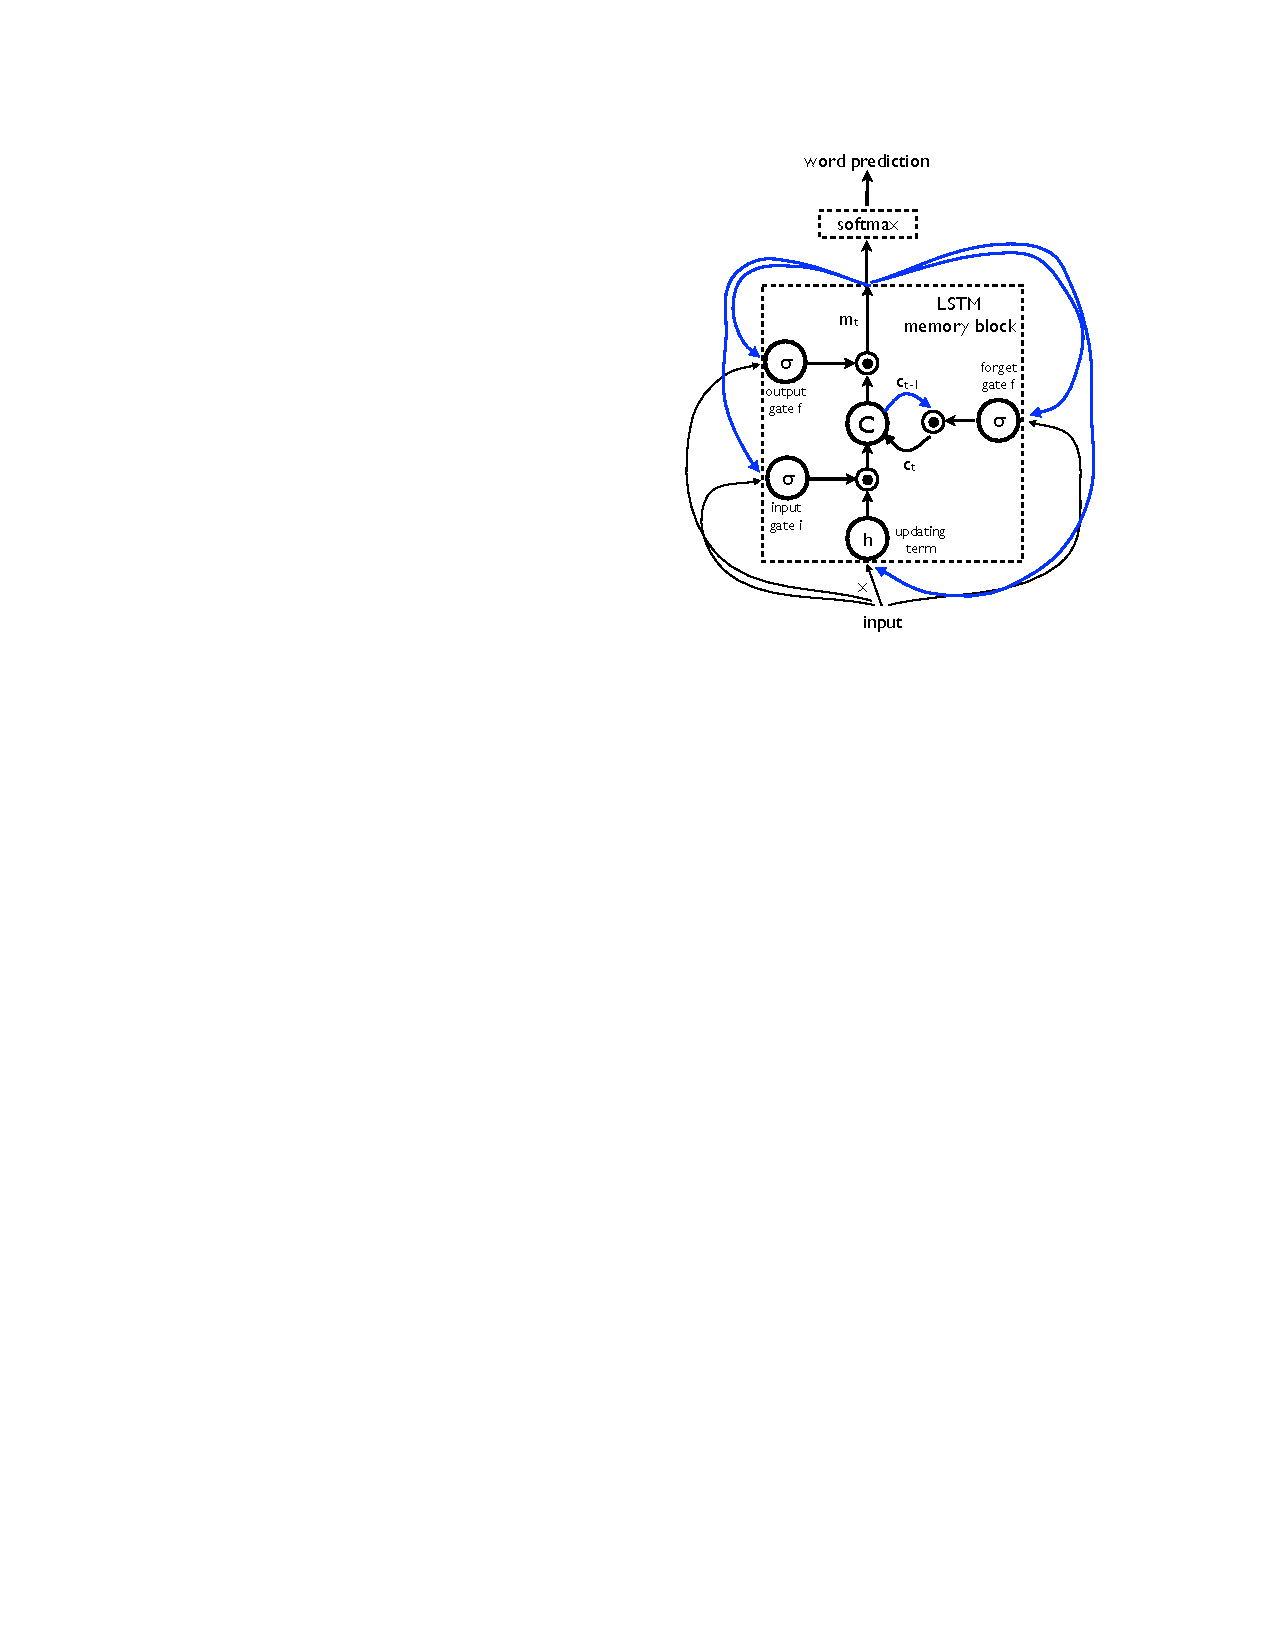
\includegraphics[width=0.5\textwidth]{images/LSTM}
	\caption{Illustration of an LSTM model adopted from \cite{vinyals2014show}: Memory cell $C$ which is controlled by three gates $\sigma_{output}$, $\sigma_{input}$ and $\sigma_{forget}$. The blue lines indicate the recurrent connections from the output $m_{t-1}$ back to the gates at time $t$.}
	\label{fig:lstm}
\end{figure}

The image $I$ is fed into the model as input $x$ only at the initial step. After this step the sequence of words in the ground truth sentence $S = (S_1,\ldots,S_N)$ is the input of the model. To mark the start and the ending of the sentence, $S_0$ and $S_{N+1}$ are special tokens. The words in the sentence are encoded as a 1-of-$K$ binary vector, where $K$ is the number of words in the entire vocabulary (training set) and there is only a single 1 on the index of the word in the vocabulary.

\begin{equation}\label{eq:loss-function-lstm}
	L(I,S)=-\sum\limits_{t=1}^{N}\log p_t(S_t)
\end{equation}

The output of the model is a probability distribution $p_t$ over all words in the vocabulary. Finally, the loss function formalized in Equation~\ref{eq:loss-function-lstm} is minimized taking into account all the parameters of the model, the image features from the CNN and the word encodings.
